\documentclass[
	12pt,
	]{article}
		\usepackage{xcolor}
			\usepackage[dvipsnames]{xcolor}
			\usepackage[many]{tcolorbox}
		\usepackage{changepage}
		\usepackage{titlesec}
		\usepackage{caption}
		\usepackage{mdframed, longtable}
		\usepackage{mathtools, amssymb, amsfonts, amsthm, bm,amsmath} 
		\usepackage{array, tabularx, booktabs}
		\usepackage{graphicx,wrapfig, float, caption}
		\usepackage{tikz,physics,cancel, siunitx, xfrac}
		\usepackage{graphics, fancyhdr}
		\usepackage{lipsum}
		\usepackage{xparse}
		\usepackage{thmtools}
		\usepackage{mathrsfs}
		\usepackage{undertilde}
		\usepackage{dutchcal}
		\usepackage{tikz}
		\usepackage{fullpage}
		\usepackage[labelfont=bf]{caption}
	\newcommand{\td}{\text{dim}}
	\newcommand{\tvw}{T : V\xrightarrow{} W }
	\newcommand{\ttt}{\widetilde{T}}
	\newcommand{\ex}{\textbf{Example}}
	\newcommand{\aR}{\alpha \in \mathbb{R}}
	\newcommand{\abR}{\alpha \beta \in \mathbb{R}}
	\newcommand{\un}{u_1 , u_2 , \dots , n}
	\newcommand{\an}{\alpha_1, \alpha_2, \dots, \alpha_2 }
	\newcommand{\sS}{\text{Span}(\mathcal{S})}
	\newcommand{\sSt}{($\mathcal{S}$)}
	\newcommand{\la}{\langle}
	\newcommand{\ra}{\rangle}
	\newcommand{\Rn}{\mathbb{R}^{n}}
	\newcommand{\R}{\mathbb{R}}
	\newcommand{\Rm}{\mathbb{R}^{m}}
	\usepackage{fullpage, fancyhdr}


	\usepackage{mathtools}
	\DeclarePairedDelimiter{\norm}{\lVert}{\rVert}
	\newcommand{\vectorproj}[2][]{\textit{proj}_{\vect{#1}}\vect{#2}}
	\newcommand{\vect}{\mathbf}
	\newcommand{\uuuu}{\sum_{i=1}^{n}\frac{<u,u_i}{<u_i,u_i>} u_i}
	\newcommand{\B}{\mathcal{B}}
	\newcommand{\Ss}{\mathcal{S}}
	
	\newtheorem{theorem}{Theorem}[section]
	\theoremstyle{definition}
	\newtheorem{corollary}{Corollary}[theorem]
	\theoremstyle{definition}
	\newtheorem{lemma}[theorem]{Lemma}
	\theoremstyle{definition}
	\newtheorem{definition}{Definition}[section]
	\theoremstyle{definition}
	\newtheorem{Proposition}{Proposition}[section]
	\theoremstyle{definition}
	\newtheorem*{example}{Example}
	\theoremstyle{example}
	\newtheorem*{note}{Note}
	\theoremstyle{note}
	\newtheorem*{remark}{Remark}
	\theoremstyle{remark}
	\newtheorem*{example2}{External Example}
	\theoremstyle{example}
	
	\title{PHYS 241 Lab 4.}
	\titleformat*{\section}{\LARGE\normalfont\fontsize{12}{12}\bfseries}
	\titleformat*{\subsection}{\Large\normalfont\fontsize{10}{15}\bfseries}
	\author{Mihail Anghelici 260928404 \\ Section  22524 Thursday\\ \\ Experiment performed with Guillaume Payeur and data collected from the TAs}
	\date{\today}
	
	\relpenalty=9999
			\binoppenalty=9999
		
			\renewcommand{\sectionmark}[1]{%
			\markboth{\thesection\quad #1}{}}
			
			\fancypagestyle{plain}{%
			  \fancyhf{}
			  \fancyhead[L]{\rule[0pt]{0pt}{0pt} Lab $4$} 
			  \fancyhead[R]{\small Mihail Anghelici $260928404$} 
			  \fancyfoot[C]{-- \thepage\ --}
			  \renewcommand{\headrulewidth}{0.4pt}}
			\pagestyle{plain}
			\setlength{\headsep}{1cm}
	\captionsetup{margin =1cm}
	\begin{document}
	\maketitle
		\section*{Question 1.}
		\vspace{-1cm}
			\begin{figure}[H]
				\centering
				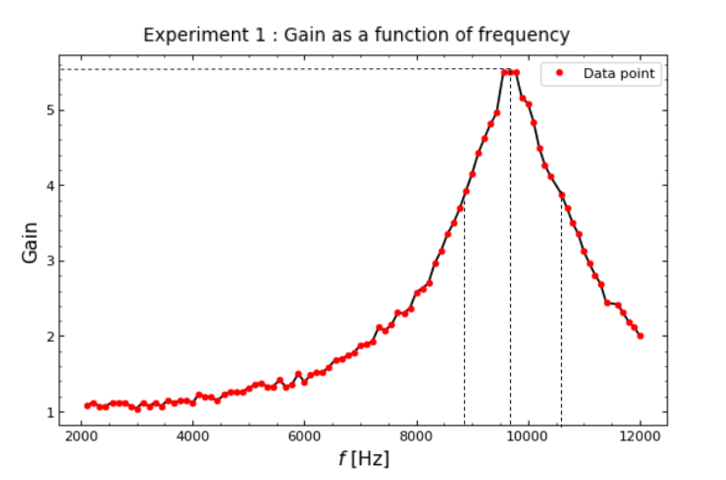
\includegraphics[width=0.7\linewidth]{PHYS241_Lab4_Exp1.png}
				\captionsetup{margin=1cm}
				\caption{Resonance plot corresponding to the experimental data gathered in Experiment 1.}
			\end{figure}
			From Figure 1, the value of $Q$ was numerically computed and found to be $\approx \ 5.59$. From this value, we may immediately compute a value for the equivalent resistance.
			\begin{align*}
				\frac{1}{Q} = \frac{R_s + r}{\omega_{0}L} \implies R_s + r &= \frac{\omega_{0}L}{Q} \\
				&= \sqrt{\frac{L}{C}}\left(\frac{1}{Q}\right)\\
				&= \sqrt{\frac{48.9 \ \cross 0.001}{4.81 \ \cross 10^{-9}}}\left(\frac{1}{5.59}\right) = 570.4 \ \si{\ohm}
			\end{align*}
			The latter value is larger of approximately $100 \ \si{\ohm}$ compared to the real resistance ,as measured with the multimeter upon the circuit's components. This is explained by the over presence of micro-sources of additional resistance within the setup up such as the co-ax cable, the solid core wires from the breadboard and the individual breadboard traces.
			
		\section*{Question 2.}
		\begin{figure}[H]
						\centering
						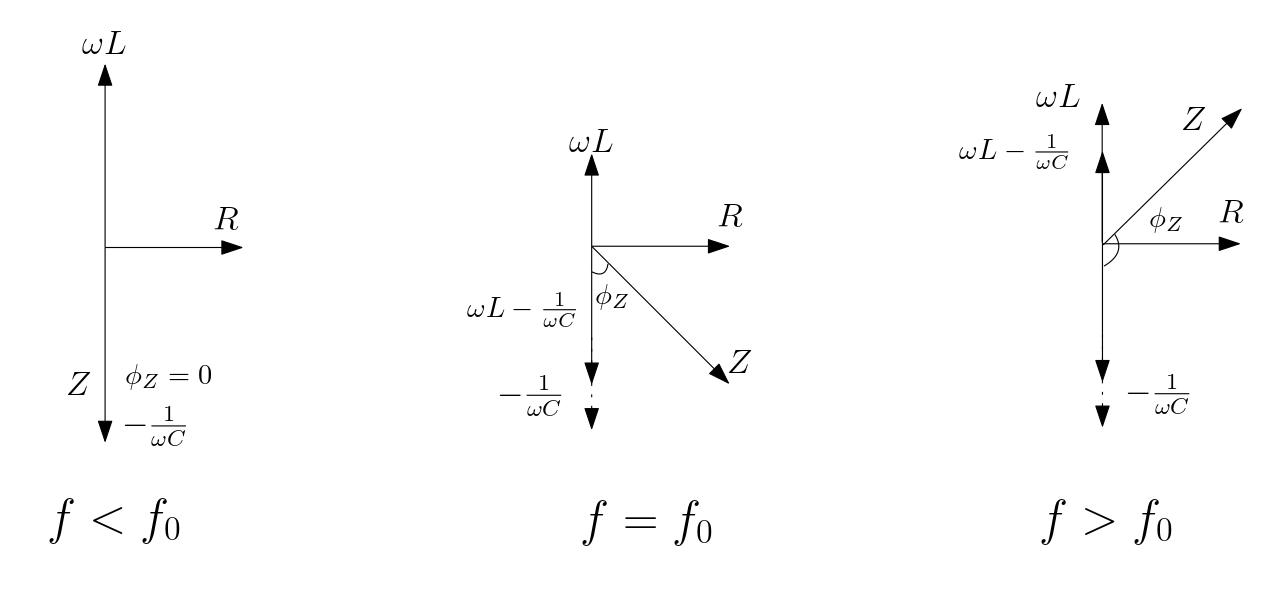
\includegraphics[width = 0.9\linewidth]{PHYS241_Lab4_VecDiagram.png}
						\captionsetup{margin=1cm}
						\caption{Vector diagram for Experiment $1$ involving impedance. The diagram presented is not fully to scale.}
					\end{figure} 
		From Figure 2, we note that for frequencies lower than $f_{0}$, the phase approaches $0$. When $f=f_{0}$ the phase is exactly $-\pi / 2$ and finally at $f > f_{0}$ we have $\varphi$ approaching  $-\pi$.
		\section*{Question 3.}
		 	The values of $Q$ were estimated graphically from the plots of Experiment 2a and Experiment 2b (Appendix A). 
		 	\begin{itemize}
		 		\item Parallel : $Q \approxeq 29.14$ 
		 		\item Series : $Q \approxeq 11.86$
		 	\end{itemize}
		\section*{Question 4.}
			\begin{gather*}
				Z_{res} = \frac{L}{Cr} = R_p \implies R_p r = \frac{L}{C}
				\intertext{Since $\omega_{0} \frac{1}{\sqrt{LC}}$,}
				R_p r = \omega_{0}^{2}L^{2} \implies \frac{R_{p}}{\omega_{0}L} = \frac{\omega_{0}L}{r} 
				\intertext{Finally, since $Q = \frac{\omega_{0}L}{r}$ as defined, then}
				\therefore Q = \frac{R_{p}}{\omega_{0}L}.
			\end{gather*}
			
		\section*{Question 5.}
			In Experiment 2a, the circuit acts like a voltage divider. The maximal gain was evaluated graphically using \textit{numpy.max()}, at $0.0965$. Then,
			\begin{gather*}
				\frac{V_{\text{out}}}{V_{\text{in}}} = \frac{R_p}{R_s + R_p} \implies R_p = R_s \left(\frac{1}{\frac{V_{\text{in}}}{V_{\text{out}}} -1}\right) \\
				\therefore R_p = 1.19 \ \si{\mega\ohm} \left(\frac{1}{(0.0964^{-1}) -1}\right) = 126.954 \ \si{\kilo\ohm}.
			\end{gather*}
			Adding a resistor of $49.8 \ \si{\kilo\ohm}$ in parallel with $R_p$ we may immediately find a value for $Q$ in Experiment 2b,
			\begin{gather*}
				R_{p,eq}  = \left(\frac{1}{R_p} + \frac{1}{49.8 \ \si{\kilo\ohm}}\right)^{-1} = \left(\frac{1}{126. 954 \ \si{\kilo\ohm}} + \frac{1}{49.8 \ \si{\kilo\ohm}}\right)^{-1} = 35.769 \ \si{\kilo\ohm}.\\
				\text{Since } \ Q = \frac{R_{p,eq}}{\omega_{0}L} \implies \sqrt{\frac{C}{L}}R_{p,eq} = Q \\
				\sqrt{\frac{4.81 \ \si{\nano\farad}}{48.9 \ \si{\milli\henry}}}(35.769 \ \si{\kilo\ohm}) = 11.218
			\end{gather*}
			This result is in excellent agreement with the experimental result ($11.208$). The experimental data had inevitable noise which in return adds uncertainty on the Gain$_{\text{max}}$ ,such that nevertheless there exists a small difference between the two latter values.
		\section*{Question 6.}
			The exponential decay factor is given by $e^{\frac{-r}{2L}t}$ , such that the amplitude scales as $I(t) = I_{0}e^{\frac{-r}{2L}t}$. We then have at $I(t)/e$, 
			\begin{gather*}
				\frac{I(t)}{e} = I_{0}e^{\frac{-r}{2L}t} \implies \frac{1}{e} = e^{\frac{-r}{2L}t} \\
				\ln(1) = \frac{-r}{2L}t+1 \implies 1= \frac{r}{2L}t.
				\intertext{Since $Q = \frac{\omega_{0}L}{r}, \implies \frac{r}{L} = \frac{\omega_{0}}{Q}$, so then}
				Q = \frac{\omega_{0}}{2} t = \frac{2\pi f_{0}}{2}t = \pi f_{0} t
				\intertext{Letting $N = t/T$ the number of cycles and $f_{0} = 1/T$ , we obtain}
				Q = \frac{\pi t}{T} = \pi N.
			\end{gather*}
			We may now use this formula to compute a value of $Q$ from the graphs observed in the ringing experiments. Because in any case, the scope's resolution is fixed and there is noise and fluctuation in the perceived plot the number of cycles could not have been accurately determined. Therefore, an average was taken between a potential range of cycles and an uncertainty computed respectively.
			\begin{itemize}
				\item Experiment 2a : $Q \approxeq 12.5 \pi \approxeq 39.3 \pm 1.6.$
				\item Experiment 2b : $Q \approxeq 3.5 \pi \approxeq 11.0 \pm 1.6.$
			\end{itemize}
			When comparing the latter values with the quality factors found in Question 3, we notice there's a substantial difference between the values of $Q$ for Experiment 2a. This is expected since the curve for that experiment is narrow. Moreover, in that experiment an insufficient number of data points were taken around $f_{0}$, such that there's an uncertainty on that value but also uncertainty on $\text{Gain}_{\text{max}}$ which in return adds error on $\Delta x$ scaling with $\sqrt{x_{1}^2 + x_{2}^2}$. Combining all these uncertainties yields a quite inaccurate value of $Q$, which is why we perceive such a large discrepancy between the two values. On another hand, the quality factors found in Experiment 2b are in good agreement which is also expected given the number of data points taken around $f_{0}$. 
		\newpage
		\appendix
		\section*{Appendix A }
		\begin{figure}[H]
										\centering
										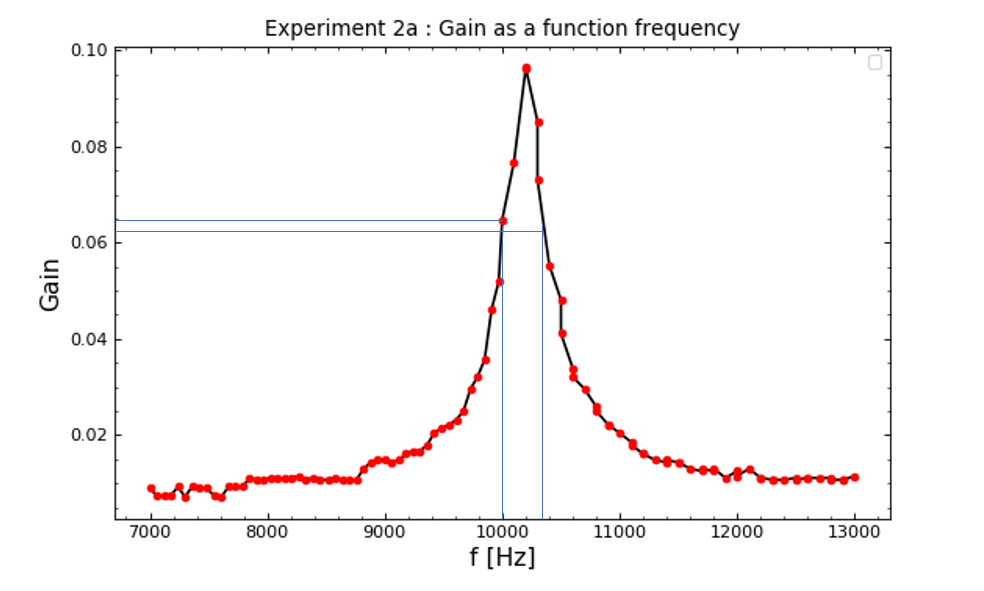
\includegraphics[width = 0.8\linewidth]{PHYS241_Lab4_Exp2.png}
										\captionsetup{margin=1cm}
										\caption{(\textbf{no-spoiler}) Experimental plot for gain as a function of frequency in Experiment 2a.}
									\end{figure} 
				\begin{figure}[H]
										\centering
										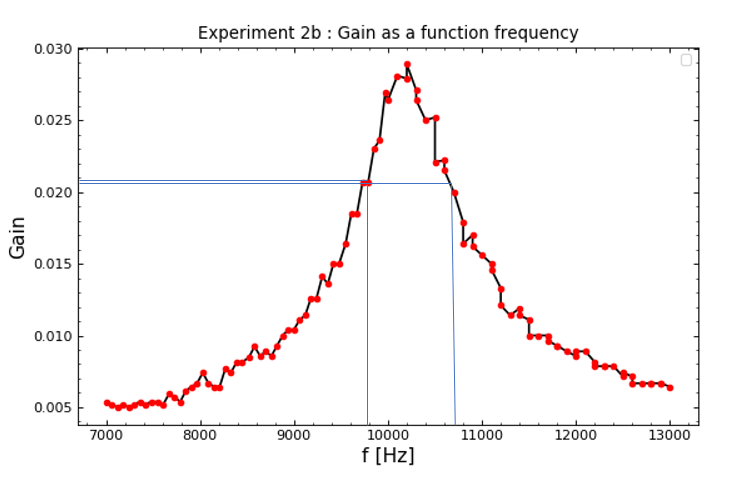
\includegraphics[width = 0.8\linewidth]{PHYS241_Lab4_Exp2b.png}
										\captionsetup{margin=1cm}
										\caption{(\textbf{spoiler}) Experimental plot for gain as a function of frequency in Experiment 2b.}
									\end{figure} 
		\newpage 
		\section*{Appendix B }
		\begin{longtable}{cccccc}
				\toprule
				\toprule
				\multicolumn{6}{c}{Raw Data} \\
				\multicolumn{2}{c}{Experiment 1} & \multicolumn{2}{c}{Experiment 2a} & 
				\multicolumn{2}{c}{Experiment 2b}\\
				\cmidrule(lr){1-2} \cmidrule(l){3-4}\cmidrule(l){5-6}
				Frequency($f$) & Gain &
				Frequency($f$) & Gain & Frequency($f$) & Gain\\
				$[\si{\hertz}]$ & & $[\si{\hertz}]$ & & $[\si{\hertz}]$&  \\
				\endfirsthead
				\multicolumn{6}{c}{Raw Data} \\\multicolumn{2}{c}{Experiment 1} & \multicolumn{2}{c}{Experiment 2a} & 
				\multicolumn{2}{c}{Experiment 2b}\\
				\cmidrule(lr){1-2} \cmidrule(l){3-4}\cmidrule(l){5-6}
				Frequency($f$) & Gain &
				Frequency($f$) & Gain & Frequency($f$) & Gain\\
				$[\si{\hertz}]$ & & $[\si{\hertz}]$ & & $\si{\hertz}$&  \\
				\endhead
				\hline \multicolumn{6}{|r|}{{Continued on next page}} \\ \hline
				\endfoot
				
				\hline \hline
				\endlastfoot
				
				\midrule
				$1000.00$&	$3.12$&	$7000.00$&	$0.01$&	$7000.00$&	$0.01$\\		
				$1111.11$&	$1.00$&	$7060.61$&	$0.01$&	$7060.61$&	$0.01$\\
				$1222.22$&	$1.04$&	$7121.21$&	$0.01$&	$7121.21$&	$0.01$\\
				$1333.33$&	$0.96$&	$7181.82$&	$0.01$&	$7181.82$&	$0.01$\\
				$1444.44$&	$1.04$&	$7242.42$&	$0.01$&	$7242.42$&	$0.01$\\
				$1555.56$&	$1.04$&	$7303.03$&	$0.01$&	$7303.03$&	$0.01$\\
				$1666.67$&	$1.04$&	$7363.64$&	$0.01$&	$7363.64$&	$0.01$\\
				$1777.78$&	$1.08$&	$7424.24$&	$0.01$&	$7424.24$&	$0.01$\\
				$1888.89$&	$1.12$&	$7484.85$&	$0.01$&	$7484.85$&	$0.01$\\
				$2000.00$&	$1.12$&	$7545.45$&	$0.01$&	$7545.45$&	$0.01$\\
				$2111.11$&	$1.08$&	$7606.06$&	$0.01$&	$7606.06$&	$0.01$\\
				$2222.22$&	$1.12$&	$7666.67$ &  $0.01$&	$7666.67$&	$0.01$\\
				$2333.33$&	$1.07$&	$7727.27$&	$0.01$&	$7727.27$&	$0.01$\\
				$2444.44$&	$1.07$&	$7787.88$&	$0.01$&	$7787.88$&	$0.01$\\
				$2555.56$&	$1.12$&	$7848.48$&	$0.01$&	$7848.48$&	$0.01$\\
				$2666.67$&	$1.12$&	$7909.09$&	$0.01$&	$7909.09$&	$0.01$\\
				$2777.78$&	$1.12$&	$7969.70$&	$0.01$&	$7969.70$&	$0.01$\\
				$2888.89$&	$1.07$&	$8030.30$&	$0.01$&	$8030.30$&	$0.01$\\
				$3000.00$&	$1.04$&	$8090.91$&	$0.01$&	$8090.91$&	$0.01$\\
				$3111.11$&	$1.12$&	$8151.52$&	$0.01$&	$8151.52$&	$0.01$\\
				$3222.22$&	$1.07$&	$8212.12$&	$0.01$&	$8212.12$&	$0.01$\\
				$3333.33$&	$1.12$&	$8272.73$&	$0.01$&	$8272.73$&	$0.01$\\
				$3444.44$&	$1.07$&	$8333.33$&	$0.01$&	$8333.33$&	$0.01$\\
				$3555.56$&	$1.15$&	$8393.94$&	$0.01$&	$8393.94$&	$0.01$\\
				$3666.67$&	$1.11$&	$8454.55$&	$0.01$&	$8454.55$&	$0.01$\\
				$3777.78$&	$1.15$&	$8515.15$&	$0.01$&	$8515.15$&	$0.01$\\
				$3888.89$&	$1.15$&	$8575.76$&	$0.01$&	$8575.76$&	$0.01$\\
				$4000.00$&	$1.11$&	$8636.36$&	$0.01$&	$8636.36$&	$0.01$\\
				$4111.11$&	$1.23$&	$8696.97$&	$0.01$&	$8696.97$&	$0.01$\\
				$4222.22$&	$1.19$&	$8757.58$ & $0.01$&	$8757.58$&	$0.01$\\
				$4333.33$&	$1.19$&	$8818.18$&	$0.01$&	$8818.18$&	$0.01$\\
				$4444.44$&	$1.14$&	$8878.79$&	$0.01$&	$8878.79$&	$0.01$\\
				$4555.56$&	$1.22$&	$8939.39$ &  $0.01$&	$8939.39$&	$0.01$\\
				$4666.67$&	$1.26$&	$9000.00$&	$0.01$&	$9000.00$&	$0.01$\\
				$4777.78$&	$1.26$&	$9060.61$&	$0.01$&	$9060.61$&	$0.01$\\
				$4888.89$&	$1.26$&	$9121.21$ &  $0.01$&	$9121.21$&	$0.01$\\
				$5000.00$&	$1.31$&	$9181.82$&	$0.02$&	$9181.82$&	$0.01$\\
				$5111.11$&	$1.35$&	$9242.42$&	$0.02$&	$9242.42$&	$0.01$\\
				$5222.22$&	$1.38$&	$9303.03$&	$0.02$&	$9303.03$&	$0.01$\\
				$5333.33$&	$1.33$&	$9363.64$&	$0.02$&	$9363.64$&	$0.01$\\
				$5444.44$&	$1.33$&	$9424.24$&	$0.02$&	$9424.24$&	$0.02$\\
				$5555.56$&	$1.42$&	$9484.85$&	$0.02$&	$9484.85$&	$0.02$\\
				$5666.67$&	$1.32$&	$9545.45$&	$0.02$&	$9545.45$&	$0.02$\\
				$5777.78$&	$1.36$&	$9606.06$&	$0.02$&	$9606.06$&	$0.02$\\
				$5888.89$&	$1.50$&	$9666.67$&	$0.03$&	$9666.67$&	$0.02$\\
				$6000.00$&	$1.39$&	$9727.27$&	$0.03$&	$9727.27$&	$0.02$\\
				$6111.11$&	$1.48$&	$9787.88$&	$0.03$&	$9787.88$&	$0.02$\\
				$6222.22$&	$1.52$&	$9848.48$&	$0.04$&	$9848.48$&	$0.02$\\
				$6333.33$&	$1.52$&	$9909.09$&	$0.05$&	$9909.09$&	$0.02$\\
				$6444.44$&	$1.59$&	$9969.70$&	$0.05$&	$9969.70$&	$0.03$\\
				$6555.56$&	$1.69$&	$10030.30$&	$0.06$&	$10030.30$&	$0.03$\\
				$6666.67$&	$1.70$&	$10090.91$&	$0.08$&	$10090.91$&	$0.03$\\
				$6777.78$&	$1.74$&	$10151.52$&	$0.10$&	$10151.52$&	$0.03$\\
				$6888.89$&	$1.78$&	$10212.12$&	$0.10$&	$10212.12$&	$0.03$\\
				$7000.00$&	$1.88$&	$10272.73$&	$0.09$&	$10272.73$&	$0.03$\\
				$7111.11$&	$1.89$&	$10333.33$&	$0.07$&	$10333.33$&	$0.03$\\
				$7222.22$&	$1.93$&	$10393.94$&	$0.06$&	$10393.94$&	$0.03$\\
				$7333.33$&	$2.12$&	$10454.55$&	$0.05$&	$10454.55$&	$0.03$\\
				$7444.44$&	$2.07$&	$10515.15$&	$0.04$&	$10515.15$&	$0.02$\\
				$7555.56$&	$2.15$&	$10575.76$&	$0.03$&	$10575.76$&	$0.02$\\
				$7666.67$&	$2.31$&	$10636.36$&	$0.03$&	$10636.36$&	$0.02$\\
				$7777.78$&	$2.30$&	$10696.97$&	$0.03$&	$10696.97$&	$0.02$\\
				$7888.89$&	$2.37$&	$10757.58$&	$0.03$&	$10757.58$&	$0.02$\\
				$8000.00$&	$2.58$&	$10818.18$&	$0.03$&	$10818.18$&	$0.02$\\
				$8111.11$&	$2.63$&	$10878.79$&	$0.02$&	$10878.79$&	$0.02$\\
				$8222.22$&	$2.70$&	$10939.39$&	$0.02$&	$10939.39$&	$0.02$\\
				$8333.33$&	$2.96$&	$11000.00$&	$0.02$&	$11000.00$&	$0.02$\\
				$8444.44$&	$3.12$&	$11060.61$&	$0.02$&	$11060.61$&	$0.02$\\
				$8555.56$&	$3.35$&	$11121.21$&	$0.02$&	$11121.21$&	$0.01$\\
				$8666.67$&	$3.50$&	$11181.82$&	$0.02$&	$11181.82$&	$0.01$\\
				$8777.78$&	$3.69$&	$11242.42$&	$0.02$&	$11242.42$&	$0.01$\\
				$8888.89$&	$3.92$&	$11303.03$&	$0.01$&	$11303.03$&	$0.01$\\
				$9000.00$&	$4.15$&	$11363.64$&	$0.01$&	$11363.64$&	$0.01$\\
				$9111.11$&	$4.42$&	$11424.24$&	$0.01$&	$11424.24$&	$0.01$\\
				$9222.22$&	$4.62$&	$11484.85$&	$0.01$&	$11484.85$&	$0.01$\\
				$9333.33$&	$4.81$&	$11545.45$&	$0.01$&	$11545.45$&	$0.01$\\
				$9444.44$&	$4.96$&	$11606.06$&	$0.01$&	$11606.06$&	$0.01$\\
				$9555.56$&	$5.50$&	$11666.67$&	$0.01$&	$11666.67$&	$0.01$\\
				$9666.67$&	$5.50$&	$11727.27$&	$0.01$&	$11727.27$&	$0.01$\\
				$9777.78$&	$5.50$&	$11787.88$&	$0.01$&	$11787.88$&	$0.01$\\
				$9888.89$&	$5.16$&	$11848.48$&	$0.01$&	$11848.48$&	$0.01$\\
				$10000.00$&	$5.08$&	$11909.09$&	$0.01$&	$11909.09$&	$0.01$\\
				$10111.11$&	$4.84$&	$11969.70$&	$0.01$&	$11969.70$&	$0.01$\\
				$10222.22$&	$4.50$&	$12030.30$&	$0.01$&	$12030.30$&	$0.01$\\
				$10333.33$&	$4.27$&	$12090.91$&	$0.01$&	$12090.91$&	$0.01$\\
				$10444.44$&	$4.12$&	$12151.52$&	$0.01$&	$12151.52$&	$0.01$\\
				$10555.56$&	$3.88$&	$12212.12$&	$0.01$&	$12212.12$&	$0.01$\\
				$10666.67$&	$3.69$& $12272.73$&	$0.01$&	$12272.73$&	$0.01$\\
				$10777.78$&	$3.50$&	$12333.33$&	$0.01$&	$12333.33$&	$0.01$\\
				$10888.89$&	$3.35$&	$12393.94$&	$0.01$&	$12393.94$&	$0.01$\\
				$11000.00$&	$3.12$&	$12454.55$&	$0.01$&	$12454.55$&	$0.01$\\
				$11111.11$&	$2.96$&	$12515.15$&	$0.01$&	$12515.15$&	$0.01$\\
				$11222.22$&	$2.81$&	$12575.76$&	$0.01$&	$12575.76$&	$0.01$\\
				$11333.33$&	$2.69$&	$12636.36$&	$0.01$&	$12636.36$&	$0.01$\\
				$11444.44$&	$2.44$&	$12696.97$&	$0.01$&	$12696.97$&	$0.01$\\
				$11555.56$&	$2.42$&	$12757.58$&	$0.01$&	$12757.58$&	$0.01$\\
				$11666.67$&	$2.31$&	$12818.18$&	$0.01$&	$12818.18$&	$0.01$\\
				$11777.78$&	$2.19$&	$12878.79$&	$0.01$&	$12878.79$&	$0.01$\\
				$11888.89$&	$2.12$&	$12939.39$&	$0.01$&	$12939.39$&	$0.01$\\
				$12000.00$&	$2.00$&	$13000.00$&	$0.01$&	$13000.00$	&$0.01$
				\end{longtable}
		
	\end{document}